\documentclass[11pt, oneside]{article}   	% use "amsart" instead of "article" for AMSLaTeX format
\usepackage{geometry}                		% See geometry.pdf to learn the layout options. There are lots.
\geometry{
	paperwidth=6in,
	paperheight=9in
	}                   		% ... or a4paper or a5paper or ... 
%\geometry{portrait}                		% Activate for rotated page geometry
%\usepackage[parfill]{parskip}    		% Activate to begin paragraphs with an empty line rather than an indent
\usepackage{graphicx}				% Use pdf, png, jpg, or eps§ with pdflatex; use eps in DVI mode
								% TeX will automatically convert eps --> pdf in pdflatex		
\usepackage{amssymb}
\usepackage{amsmath}
\usepackage{authblk}
\usepackage{graphicx}

\usepackage{url}
\usepackage{hyperref}
\usepackage{breakurl}

%SetFonts
\newenvironment{defenseinfo}[1][10em]
  {\noindent\begin{tabular}{@{}l@{~\makebox[#1]}}}
  {\end{tabular}}
%SetFonts
\title{Defining Ecosystem Boundaries within a Stable, Diverse and Extensive Alarm Management Platform\\
\\
A Manifesto for Systems Architecture}
\author{A T Parkinson}							% Activate to display a given date or no date

\begin{document}

\pagebreak
\pagebreak

\maketitle
  \\
\vfill
\begin{center}
Fringe Papers: Wedmore, Somerset, UK.\\
  \end{center}

\pagebreak

\vspace{5mm}

\vfill

\begin{defenseinfo}

https://github.com/realfeed/manifesto is in the public domain.\\
\\
First Edition 2023\\
\\
ISBN: [PUBLICATION ISBN NUMBER] (hardback)\\
\\
Visit the authors website at https://aidanparkinson.xyz\\
\\
Fringe Papers is a registered trademark of Realfeed Ltd.\\
\\
\end{defenseinfo}

\pagebreak

\section*{Abstract}
It has been recognised the the prevailing discussion on the governance of platform ecosystems may have contributed to global ecosystem instability in alarming ways.
The prioritisation of network effects to deliver a popular market share of consumers tends to be a common Feature.
This investigation seeks to diagnose causes of instability and define new platform ecosystem boundaries for more stable outcomes.
It is understood that this has been achieved through an investigation of ethics, continuous integration processes and operations.
This investigation appreciates the differences between the \emph{states} of Locke and \emph{State} of Hobbes.
The Sovereignty of states and their role in forming civil society are recognised and this platform submits to the necessary assurance regime of a state.
However, a significant difference of this platform ecosystem to others is the acknowledgement that a society need also submit to a global Sovereign of State which accounts for the condition of the Earth's ecosystem.
What follows is the use of a Hobbesian Commonwealth Cost of Carbon as an overall quality of life indicator and a Rawlsian process of alarm management.\
The resulting \emph{Commonwealth of Peoples} could adopt traditional principles of justice amongst free and democratic peoples without conflict.
Complimenters are encouraged to develop their own Features for integration with this ethical Framework.
A minimal set of criteria has been identified for complimenters to develop new Features for end-consumers.
Although these criteria are not nearly complete at this point of time, it is hoped that they prove a stable enough starting point to generate interest.\
In operation the platform is to share knowledge in concert with other Professionals to develop mutually assured approaches in Good faith.
Licensing of Property is highly permissive to support conditions of fair liberty and equality of opportunity.

\pagebreak

\section{Introduction}
Digital platform governance involves thoughtful considerations towards the standardisation of interfaces to enable a diverse market of complimenters to find opportunity in developing Features for consumers.
There has been much discussion about the creation of platforms that prioritise network effects to deliver a popular market share of consumers with compelling development opportunities for complimenters to offer proprietary tools to enhance personal utility.
Such an approach has been very successful for exploiting new domains, such as the internet and personal client devices~\cite{bop1}.
However, such contributions may be somewhat detrimental in addressing societies pressing contractual problems involved in minimum security Standards to govern a limited natural ecosystem.
Loss of biodiversity, the coercive politics of limiting global temperature rise, social unrest and military intervention are all relevant demonstrations in this domain and appear to exhibit some common Features.\

One potential area of conflict in ecosystem governance is the management of competing principles of what is Good.
This involves a definition that not only justifies ecosystem ethical priorities, but also a recognition of what is Sovereign.
Minimal policies could then be identified to contribute towards ecosystem stability and align supply-chains with a natural course of development.\

Another important aspect is to set boundaries for the development of distinctive attributes known as \emph{Features}.
Frameworks and Guidance need identifying that signal the failure of Features under development within an environment that supports continuous integration.
Failure is an important feedback mechanism for developers to learn and adapt work-in-progress Features and, hence, enforcement need ideally to be rapid, consistent and relevant.
It has been recognised that practical networking of outstations and sensors in the field with public domains has historically been poorly enforced.
Lack of consumer confidence has contributed to sluggish market penetration of internet-of-things technologies to-date.\

Further, it appears important to consider the management of Property and how governing agents may operate.
Such thought needs to reflect on the ecosystems ethical priorities, competition and operational costs.\

Therefore, this article asks the question:\\

\emph{How could one govern an alarm management platform to support a stable and diverse natural ecosystem?}\\

The discussion draws upon experience of practice and a wide-ranging review of theory.
In conclusion an Ontology that offers the authors perspective on this question is proposed.
It is acknowledged that the problems faced are formidable and no solution can be perfect.
However, it is intended that this article contributes common-sense that may inspire the sustainable development of new technologies going forward.\

\pagebreak

\section{Ethics}
It is acknowledged that any ecosystem may include agents with different interests and potentially competing principles of what is Good.
However, it is extremely challenging to identify a global perspective of what a Good interest is.
In an attempt to govern a natural ecosystem, one could understand that a process of identification involves considering prevailing representations of the State of Nature.
Two influential accounts define significantly different interpretations of nature and association.
These are John Locke Second Treatise and Thomas Hobbes' Leviathan.
This document carefully draws distinctions between these two perspectives by use of the terms \emph{states} and \emph{State}\

John Locke defines a \emph{state} of nature for individuals~\cite{jl1}.

\begin{quote}
"...a state of perfect freedom to order their actions and dispose of their possessions and persons as they think fit, within the bounds of the law of nature, without asking leave or dependency on the will of any other man."
\end{quote}

Locke then defines bounds of nature~\cite{jl1}.

\begin{quote}
"...no one ought to harm another life, health, liberty or possessions."
\end{quote}

From Locke's perspective, some persons may transgress these bounds and in response people may defend themselves or others against such invaders of rights.
The injured party and his agents may then recover from the offender~\cite{jl1}.

\begin{quote}
"...so much as may make satisfaction for the harm suffered"...
\end{quote}
\begin{quote}
"...everyone has a right to punish the transgressors of that law to such a degree as may hinder violation."
\end{quote}

Nozick describes how such a view leads to the development of protective associations to enforce what an individual beliefs to be their rights, with others joining a call for defence.
To avoid mutually harmful conflict between protective associations, a system of appeal courts and judgements are made on jurisdiction and the conflict of laws in favour of the dominant protective association.
Protection and enforcement of people's rights is treated as an economic Good to be provided by the market, as are other important Goods such as food and clothing~\cite{rn1}.\

Alternatively, Hobbes defines a \emph{State} of nature for civil society.
Hobbes assumes all people as naturally equal in body and mind.
This includes an equality of hope in the attaining of ends.
This leads to three principle causes of quarrel: competition for personal gain; diffidence for safety; and glory for reputation. Without a common power to stipulate rules a war of all against all ensues and a potentially fraught and divisive struggle ~\cite{th1}.

\begin{quote}
"NATURE had made men so equal, in the faculties of the body and mind..."
\end{quote}
\begin{quote}
"Hereby it is manifest, that during time men live without a common power to keep them all in awe, they are in that condition which is called war; and such a war, as is of every man, against every man. For WAR, consisteth not in battle only, or the act of fighting; but in a tract of time, wherein the will to contend by battle is sufficiently known: an therefore the condition of time, is to be considered in the nature of war, as it is in the nature of weather. For as the nature of foul weather, lieth not in a shower or two of rain; but in an inclination thereto of many days together: so the nature of war, consisteth not in actual fighting, but in the known disposition thereto, during all the time there is no assurance to the contrary. All other time is PEACE."
\end{quote}
\begin{quote}
"To this war of every man against every man, this also is consequent; that nothing can be unjust. The notions of right and wrong, justice and injustice have there no place. Where there is no common power, there is no law, no injustice. Force, and fraud, are in war the two cardinal virtues. Justice, and injustice are none of the faculties neither of the body, nor mind."
\end{quote}

However, Hobbes asserts that there are certain conditions where men are inclined to peace: fear of death; desire for a certain standard of living; and hope for industry ~\cite{th1}.

\begin{quote}
"The passions that incline men to peace, are fear of death; desire of such things as are necessary to commodious living; and a hope by their industry to obtain them. And reason suggesteth convenient articles of peace, upon which men may be drawn to agreement. These articles, are they, otherwise are called the Laws of Nature..."
\end{quote}

When people mutually covenant each to the others to obey a common authority, they have established what Hobbes calls \emph{Sovereignty by institution}. When, threatened by a conqueror, they covenant for protection by promising obedience, they have established \emph{Sovereignty by acquisition}. These are equally legitimate ways of establishing Sovereignty. The social covenant involves both the renunciation or transfer of right and the authorisation of the Sovereign power. Political legitimacy depends not on how a government came to power, but only on whether it can effectively protect those who have consented to obey it; political obligation ends when protection ceases.\par

Through transferring ones personal freedoms to a trusted Sovereign one sets up the conditions for \emph{keeping of promise} and, hence, the conditions of stable currency. Such a Sovereign requires resources for enforcement to ensure performance of promises made and defend against competing externalities~\cite{th1}.

\begin{quote}
"The mutual transferring of right, is that which men call CONTRACT."
\end{quote}
\begin{quote}
"... one of the contractors, may deliver the thing contracted for on his part, and leave the other to perform his part at some determinate time after, and in the mean time be trusted: and then the contract on his part, is called PACT, or COVENANT: or both parts may contract now, to perform hereafter: in which cases, he that is to perform in time to come, being trusted, his performance is called \emph{keeping of promise}, or faith: and the failing of performance (if to be voluntary) \emph{violation of faith}."
\end{quote}
\begin{quote}
"He that transferreth any right, transferreth the means of enjoying it, as far as leith in his power. As he that selleth land, is understood to transfer the herbage, and whatsoever grows upon it; nor can he that sells. mill turn away the stream that drives it. And they that give to a man the right of government in Sovereignty, are understood to give them the right of levying money to maintain soldiers; and of appointing magistrates for the administration of justice."
\end{quote}

Hobbes prescribes peace, promise and rule of laws as a Good for social benefit as far as there is hope to obtain it~\cite{th1}.

\begin{quote}
"... that every man, ought to endeavour peace, as far as he has hope of obtaining it; and when he cannot obtain it, that he may seek, and use, all helps, and advantages of war."
\end{quote}
Through taking the Hobbesian perspective into account, we may be led to the contributions of John Rawls as a substantive governance system for managing competing principles of the Good.\

Through an exploration of conflicts between these two perspectives on the State of Nature, an Executive Function for Alarm Management proposition may be defined as follows:\

\subsection{Sovereignty}
Following our exploration of a State of Nature, we understand that identification of a Sovereign is a necessary requirement of any ecosystem to be governed.
The initial priority here is to address root cause of \emph{uncaught promises} which may result from conflicts between the prevailing perspectives of Locke and Hobbes.
It is suggested that an essential reliance on states to underwrite and re-negotiate the competing priorities of contractual obligations compromised through unexpected natural disasters entirely undermines justification of popular governance models grounded in Locke's state of nature.
Locke's bounds of nature can only conceivably apply to civil society and entirely miss the potential of the wild to bring anyone to harm.
It is unrealistic to claim freedom from having to submit to a common natural ecosystem.
A society of peoples needs to submit to a Hobbesian perspective of a Sovereign ecosystem for all humanity called \emph{Earth}.
The resulting \emph{Commonwealth of Peoples} could adopt traditional principles of justice amongst free and democratic peoples without conflict ~\cite{jr2}.\

\subsection{Quality-of-life}
\emph{Carbon} is a name for a non-metallic element with atomic number 6 and symbol C.
On Earth this element has a key role in a \emph{carbon cycle} that is essential for all forms of life on the planet.
This cycle involves exchanges of carbon-based vapours with the Earth's atmosphere.
Plants sequester Carbon Dioxide (CO\textsubscript{2}) through photosynthesis.
Animals and plants emit CO\textsubscript{2} and animals Methane (CH\textsubscript{4}) through respiration and metabolic processes.
Industrial processes can also emit CO\textsubscript{2} and other carbon-based vapours to deliver Goods and services to support a growing human populations well-being~\cite{ng1}.\

There is evidence of a governance problem with the carbon cycle on Earth from the British Antarctic Survey.
The British Antarctic Survey has studied ice cores and the air bubbles trapped within them from Antarctica and Greenland since the 1950’s.
Such research seeks to understand historic temperature and concentrations of molecules in the Earth’s atmosphere.
The studies provide evidence of stable concentrations of CO\textsubscript{2} since year 1000AD, until the onset of the industrial era in the early 19th century.
Since then, concentrations have risen and were reported in 2010 to be approximately 1.4 times higher than before industrialisation.
Such high concentrations of CO\textsubscript{2} in the atmosphere are thought to be unprecedented in the previous 800,000 years. Furthermore, levels of Methane (CH\textsubscript{4}) have more than doubled since the industrial era.
The studies have found evidence of a statistically significant correlation between concentrations of CO\textsubscript{2} in the Earth’s atmosphere and temperature change~\cite{ba1}.
Since the time of Tyndall, scientists have known that carbon-based vapours may absorb radiant heat, and this suggests causality~\cite{td1}.
Harvey explains how, when considering carbon-based vapours potential to absorb radiant heat it is important to consider both the degree of radiant forcing and the duration gases will remain in the atmosphere.
In doing so, one arrives at estimates of what is considered a carbon-based vapours \emph{global warming potential}~\cite{dldh1}.\

Global average near-surface temperatures have warmed by about 0.7 degrees Kelvin since 1900.
Over the past 30 years, global temperatures have risen rapidly at a rate of approximately 0.2 degrees Kelvin per decade reaching a level not experienced for about 12,000 years~\cite{hj1}.
The NASA Goddard Institute for Space Studies found in 2011 that global average surface temperature continues a trend in which nine of the 10 warmest years in the modern meteorological record at that time had occurred since the year 2000.
The study reports that the average temperature around the globe in 2011 was 0.51 degrees Kelvin warmer than their mid-20th century baseline~\cite{candm1}.
The Stern Review forecasts that further rises in global average near-surface temperatures could threaten the well-being of people across the world, predicting: the melting of glaciers; declining crop yields; ocean acidification; rising sea levels; risks of malnutrition and heat stress; permanent displacement of communities; and mass extinction of between 15-40 percent of Earth's species~\cite{ns1}.\

This means that activities undertaken privately, release carbon-based vapours that contribute to a cost born by all society globally.
A society as diverse in its tastes and interests, as political organisation.
Faced with fear for our future, even those of just intentions may be condemned to permanent hostility whilst public assurance is not forthcoming and apprehensions grow of the faithfulness of others.
Under such circumstances, Rawls asserts that as a free and rational person one has a natural duty to comply with just institutions where they apply and assist in the establishment of just arrangements where they do not exist, at least when this might be achieved with little cost to ourselves.
Along with such action comes a duty to show others mutual respect and a willingness to observe situations from their point-of-view, considering their perspective of the Good.
Further, one should be prepared to give reasons for their judgements wherever the interests of others are materially affected. In this way any proposition can be offered in Good faith, enabling others to accept constraints on conduct~\cite{jr1}.\\
\\
 \emph{How could one ensure their demands are of maximum social benefit?}\\
 \\
Coase suggests that one might need to add the costs of their greenhouse gas emissions born by all society to their own private costs when taking action.
This would correct production processes so they are of maximum social benefit~\cite{rc1}.
Precedents use the term \emph{social cost of carbon} to define the mean average costs of greenhouse gas emissions born by all society for this purpose.
However, in this context it seems there are different perspectives that may be taken towards what this social benefit may be.
An explanation of two prominent perspectives follow, the differences between them yielding significantly different outcomes for action.

\subsubsection{Notable Precedents: Utilitarian Perspective}

Calculation of a social cost of carbon has proven to be highly rewarding for those taking utilitarian perspectives, prescribing happiness as a whole as the ultimate end to action ~\cite{hs1}. The resources consumed in satisfying human needs require economic considerations to efficiently manage personal well-being. Normative economists often regard only individual circumstance, or level of  welfare, in a state of affairs as important. This is known as the neutrality assumption~\cite{pd2}. Arrow, May and Sen assert that this position of neutrality is effectively an avocation of anonymity with respect to social states, which is a requirement that human beings be treated equally~\cite{ka1}~\cite{km1}~\cite{as2}. Waldron defines the notion of social welfare, an aggregate of individual welfare, as being goal-based~\cite{jw2}. Dworkin states that a goal can be considered a non-individuated political aim~\cite{rd1}.

Early contributions to address this research question were awarded the Nobel Prize~\cite{np1} and life peerages in the House of Lords~\cite{g1}. These notable precedents prescribe aggregate or social welfare as a goal for social benefit. Aggregate welfare is not evenly distributed amongst the worlds population. In 2019, Business Insider magazine reported that the 26 richest men had more combined wealth than the poorest 3.8 billion people on Earth~\cite{bi1}. Therefore, pure reinforcement of aggregate welfare is largely in the interest of a few wealthy people. This approach typically employs Frank Ramsey's Mathematical Theory of Saving as a decision-making tool. The process involves creating complex integrated assessment models of humanities social and environmental systems that apply gross assumptions of Earth's development. Mechanisms that determine the state of the world are identified and the consequences of alternative policies charted so that consequences can be valued. Welfare surpluses are then estimated for policy options, by making projections of differences from the \emph{status quo} 100's of years into the future. Valuation of these surpluses involves setting a global social discount rate and this requires a set of personal assumptions~\cite{pd2}. A summary of the underlying decision-making criteria is shown follows~\cite{fr1}:

\begin{equation}
V_t = \sum_t^\infty \beta^{(\tau - t)} \cdot U (C_\tau)
\qquad \text{for }
\qquad t \geq 0
\end{equation}

where,
\begin{equation}
\beta = \frac{1}{(1+\mu)}
\end{equation}

Where, $V_t$ is \emph{a generations welfare}, $\beta$ is the \emph{discount factor}, $U$ is \emph{welfare}, $C_\tau$ is \emph{consumption during time-step}, $t$ is \emph{time} and $\mu$ the \emph{social discount-rate}.

\begin{equation}
\mu = \sigma \cdot g + \delta
\end{equation}

Where, $\sigma$ is the \emph{marginal utility of consumption} and the difference in the utility one would gain from a unit of consumption by those of low and high incomes, $g$ is the \emph{long-term growth rate} in consumption, $\delta$ is the \emph{pure rate of time preference} and our impatience to consume in fear of extinction.

\begin{equation}
S = \frac{\mu-\delta}{\sigma \cdot \mu}
\end{equation}

Where, $S$ is the \emph{savings rate} and the proportion of output that should be invested.\par

In practical applications, $U (C_\tau)$ can be substituted for net cash-flow in time period to yield a familiar equation.\par

This complex process results in considerable disagreement amongst social cost of carbon estimates for a historic time period using this method.
The assumptions for a global social discount rate used for three notable contributions are provided in Table 1. The global social discount rate for these three contributions ($\mu$) is similar. However Cline is outlying in estimation of the difference in utility the wealthy gain from a unit of consumption compared to the poor ($\sigma$). None of the three contributions agree on a long-term global growth rate ($g$). When considering impatience to consume in fear of extinction ($\delta$) it is Nordhaus that appears outlying. This yields very different values for the amount of surplus to be saved relative to that consumed amongst the three contributions ($S$). Clearly the worlds envisioned by just these three notable precedents are really quite different in nature and perhaps the reality is that the ethical positions of these contributors are in competition. Nobody has the power in reality to set a social discount rate in this way for all society. For most, the setting of these assumptions is of private preference only.

\begin{table}[h]
\caption{Notable precedents: assumptions in social discounting}
\begin{center}
\begin{tabular}{| l | c | c | c | c | c |}
\hline
Contribution&$\mu$&$\sigma$&$g$&$\delta$&$S$\\
\hline
Cline, 1992~\cite{wc1}&0.05&1.5&0.033&0&0.67 \\
Nordhaus, 1994~\cite{wn1}&0.05&1&0.02&0.03&0.4 \\
Stern, 2006~\cite{ns1}&0.05&1&0.049&0.001&0.98 \\
\hline
\end{tabular}
\end{center}
\label{Social contributions table}
\end{table}

Figure~\ref{USA SCC figure} is a graphical representation of social cost of carbon estimates by the Interagency Working Group on Social Cost of Carbon, United state's Government. This meta-analysis considers the results of three pioneer integrated assessment models developed in the 1990's. These are the DICE, PAGE and FUND models~\cite{wn1}~\cite{ch1}~\cite{rsjt1}. The modelling simulations considered by this study returned a social cost of carbon anywhere between $<$2007\$0tC\textsuperscript{-1} to a 95th percentile of 2007\$128tC\textsuperscript{-1} with $\mu$ set at 0.03~\cite{iwg1}. Based upon these results for a social cost of carbon, it is clear that utilitarians would find it difficult to significantly alter their actions and agree on options to be taken. 

\begin{figure}[ht]
\caption{Social Cost of Carbon in 2010 (in 2007 dollars per metric ton)}
\centering
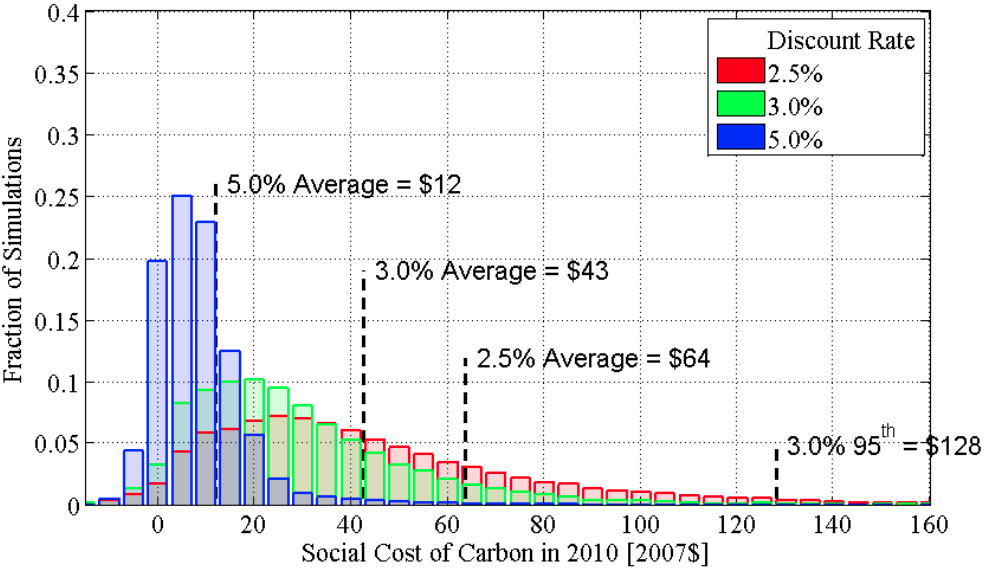
\includegraphics[width=0.7\textwidth]{scc}
\label{USA SCC figure}
\end{figure}

\begin{quote}
"Here there are a number of possibilities. A collective decision may determine the rate of saving while the direction of investment is left largely to individual firms competing for funds. In both a private Property as well as in a socialist society great concern may be expressed for preventing irreversible damages and for husbanding natural resources and preserving the environment. But again either one may do rather badly."~\cite{jr1}
\end{quote}

Even among welfare economists, some reject applying pure time preference so that one allows the living to take advantage of their position in time to favour their own interests~\cite{hs1}~\cite{fr1}. Such examples ignore the possibility for the living to wrong their predecessors or descendants. Dasgupta argues that it is one thing to urge that an imperfect economy should be improved, quite another to pretend that the imperfect economies we inhabit are Utopia in the way these contributions suggest. Collective saving for the future has many aspects of a public Good, though under conditions of arising problems of isolation and assurance~\cite{as1}~\cite{ms1}.  Those who follow the principles of the social contract when taking action would probably find these methods have little relevance to their sense of justice. These contributions also do not consider the possibility for states of affairs to deliver imperfect procedural justice leading to noncompliance. Libertarian's might argue that such collective action would lead to violations of individual rights to even a slight extent and therefore should be rejected~\cite{rn1}. Advocates of the free-market may criticise such methodologies that involve seeking prosperity through centralised long-term coercive planning, rather than appropriate regulation that allows local agents to adjust their activities according to the present situation~\cite{fh1}. There is indeed nothing sacrosanct about the public decision concerning the level of savings and its bias with respect to time preference deserves no special respect~\cite{jr1}. Therefore, an alternative proposition is sought.

\subsubsection{Proposition: Hobbesian Perspective}

An alternative perspective is to use the principles of the social contract to estimate a Commonwealth cost of carbon for decision-making.
Here, one cannot rely on the assumption that the ideals of liberal democracy or social welfare are necessarily shared by all those affected.
However, one might assume universal acknowledgement of a Hobbesian ecosystem.

The problem is to use Hobbesian thought to value the social cost of greenhouse gas emissions as a Good.
Dasgupta asserts that this valuation need involve comparison of worlds with and without greenhouse gas emissions and stable currency~\cite{pd2}.
Our understanding of the carbon cycle helps us determine that a world without greenhouse gas emissions is a world without life.
The moon is an example of a world without a significant carbon cycle.
Carbon appears an essential good life cannot do without.
Our next task is to understand what a world would be like without stable currency.
Hobbes would suggest this be a war of \emph{all against all}, a world without submission to a Sovereign power.
To maintain confidence, citizens of a well-ordered society will normally want the rule of law maintained.
Although we might acknowledge that a common sense of justice is shared and that each wants to adhere to its arrangements, one might nevertheless lack full confidence in one another.
One might suspect that others are not doing their part, and so may be tempted not to do theirs.
The general awareness of these temptations may cause social systems to break down.
The role of an authorised public interpretation of rules supported by collective sanctions is needed precisely to overcome this instability.
For this reason alone, a coercive State is always necessary, even though in a well-ordered society sanctions may be slight and may never need be imposed.
Therefore, the penal machinery of State becomes ones security to another and is entirely sacrificial~\cite{jr1}.\par

Therefore, in order to optimise ones actions to assure \emph{faith in promise} one arrives at a quality-of-life indicator equivalent to a \emph{Commonwealth Cost of Carbon} for a given time-period we complete the following calculation:

\begin{equation}
Commonwealth\; Cost\; of\; Carbon = \frac{gross\; anthropogenic\; expenditure\; on\; enforcement}{gross\; anthropogenic\; greenhouse\; emissions}
\end{equation}

It is evident that this calculation method requires relatively straightforward math, but the accounting is not trivial.
An initial anchor for the year 2016 could be arrived at through dividing public EU accounts for global military expenditure (\$1.8tn) and dividing by a Kyoto Protocol figure for global gross greenhouse gas emissions (10GtC) to arrive at \$180tC\textsuperscript{-1}~\cite{eu1}~\cite{co1}.
The genuine figure for a Commonwealth Cost of Carbon might be double this initial anchor, once global expenditure on public order and safety were added to the gross enforcement cost total, ranging somewhere between \$300tC\textsuperscript{-1} and \$400tC\textsuperscript{-1}~\cite{oecd1}.
Unfortunately, accurate figures for these expenditures remain difficult to obtain and involves considerable uncertainty.
This leads to the belief that estimation of a Commonwealth Cost of Carbon using the principles of the social contract return results of a different order of magnitude to even the higher utilitarian estimates in 2010 that average 2007\$64tC\textsuperscript{-1}  with $\mu$ set at 0.025~\cite{iwg1}.

There are a number of implications in taking a Hobbesian approach to calculating the Commonwealth Cost of Carbon which are very different from the utilitarian perspective.
Here, a Commonwealth Cost of Carbon becomes of no concern when there is no need for anyone to enforce a promise - a Hobbesian Utopia that is very difficult to achieve.
Further, maintaining enforcement costs, whilst reducing greenhouse gas emissions, increases the Commonweath Cost of Carbon for those following the principles of the social contract for the global commons.
The correction to decision-making required appears substantial and may be applied to every personal cost-based decision of anybody.
There is no reliance on an ideal observer, all peoples are treated equally and allocations of property rights have no influence on the ability of anyone to estimate.
The Hobbesian perspective does not support the view that anybody should be embargoed for their contributions to climate change.
It also does not indicate a target global mean surface temperature rise, as this is no longer the chief concern.\

It is assumed that each person reasonably believes that others have a sense of justice and an effective desire to carry out their obligations.
Without this mutual confidence, little is accomplished by uttering words.
The indivisibility and public nature of certain essential Goods, such as the element Carbon and the State of the Earth, give rise to externalities and temptations that necessitate collective agreements organised and enforced by states.
Once Goods are indivisible over large numbers of individuals, their actions decided upon in isolation from one another will not lead to the general Good.
Some collective arrangement is necessary and everyone wants assurance that it will be adhered to if willing to take part. In a large community, confidence in one another's integrity rendering enforcement superfluous is not to be expected~\cite{jr1}.
Recognition of a Commonwealth Cost of Carbon involves dealing with a system of transaction costs and might require a highly centralised intervention.
Ideally, this Commonwealth Cost of Carbon might be applied as a common rate of value-added tax on the global warming potential of delivered fuels, including food, to be excised as duty by a society.
Alternatively, the entire society could be internalised within a single non-coercive firm~\cite{rc1}.
Proportional expenditure taxes have been noted as potentially being part of a best tax scheme that treats everyone in a uniform way, with the possibility of making exemptions for dependents~\cite{nk1}.
Either option could be open using the Hobbesian approach, as the relatively simple calculation methodology involved may be an auditable record by the general public to overcome major assurance problems effecting the stability of any covenant.
A remaining challenge exists in assuring that all parties have the necessary assurance to follow through on such commitments.
This involves members giving promise and a reciprocal recognition of their intention to put themselves under an obligation that is to be honoured.
Through reciprocal recognition and common knowledge such arrangements can be enabled, started and preserved~\cite{hp1}.\

By choosing a higher and publicly auditable Commonwealth Cost of Carbon a broader range of interventions that lead to greenhouse gas abatement become viable, which may include: closer activity control to reduce waste; reduced development of excessive plant and infrastructure capacity; increased utilisation of productive assets; renewable energy sources; and active modes of transport, such as walking and cycling.
The overall effect would be to promote a society that makes solemn recognition of the great sacrifices made to maintain the current global State of affairs, observing more diligent attention to their own impacts upon the commons.\

\subsection{Minimum Decency}

Rawls'~\cite{jr1} full statement of justice for institutions is a concise and widely recognised solution to the priority problem of justice as fairness. A sense of which I wish to share and apply. An account, but not a defence, follows.

\subsubsection{First principle}

\begin{quote}
"Each person is to have an equal right to the most extensive total system of equal basic liberties compatible with a similar system of liberty for all."
\end{quote}

\subsubsection{Second principle}

\begin{quote}
"Social and economic inequalities are to be arranged so that they are both:
\begin{description}
\item[ a)] to the greatest benefit of the least advantaged, consistent with the just savings principle, and
\item[ b)] attached to offices and positions open to all under conditions of fair equality of opportunity."
\end{description}
\end{quote}

\subsubsection{First priority rule: the priority of liberty}

\begin{quote}
"The principles of justice are to be ranked in lexical order and therefore liberty can be restricted only for the sake of liberty.
There are two cases:
\begin{description}
\item[ a)] a less extensive liberty must strengthen the total system of liberty shared by all;
\item[ b)] a less than equal liberty must be acceptable to those with lesser liberty."
\end{description}
\end{quote}

\subsubsection{Second priority rule: the priority of justice over efficiency and welfare}

\begin{quote}
"The second principle of justice is lexically prior to the principle of efficiency and to that of maximising the sum of advantages; and fair opportunity is prior to the difference principle. There are two cases:
\begin{description}
\item[ a)] an inequality of opportunity must enhance the opportunities of those with the lesser opportunity;
\item[ b)] an excessive rate of saving must on balance mitigate the burden of those bearing the hardship."
\end{description}
\end{quote}

\subsubsection{General conception}

\begin{quote}
"All social primary goods---liberty and opportunity, income and wealth, and the bases of self-respect---are to be distributed equally unless an unequal distribution of any or all of these goods is to the advantage of the least favoured."
\end{quote}

\subsection{Rate of saving}

Rawls' second priority rule stipulates a requirement to control rates of saving, so that excessive rates on balance mitigate the burden of those bearing the hardship. Therefore, there is a requirement to estimate the present generations rate of saving. This returns an aggregation of the well-being of individuals, often described as \emph{intergenerational well-being}.

\subsubsection{Cost-benefit analysis}

Dasgupta~\cite{pd2} explains how we \emph{value} when comparing objects and we \emph{evaluate} when comparing the benefits of actions.
Valuation and evaluation both involve comparisons between worlds with and without the course of action or object.
This process is called social cost-benefit analysis and involves measuring consumer and producer \emph{surpluses}.
Carrying out social cost-benefit analysis requires a quantitative formulation of intergenerational well-being, for which Ramsey's Mathematical Theory of Saving~\cite{fr1} is a well respected candidate.

\subsubsection{Accounting}

To establish estimates for rates of saving it is necessary to account for circumstances with and without a course of action or object. There are a broad range of influences on well-being that need to be accounted for. Here an original convenient taxonomy is proposed in illustrated in Figure~\ref{Influences on well-being figure}, inspired somewhat by Dasgupta~\cite{pd3}.

\begin{figure}[ht]
\begin{center}
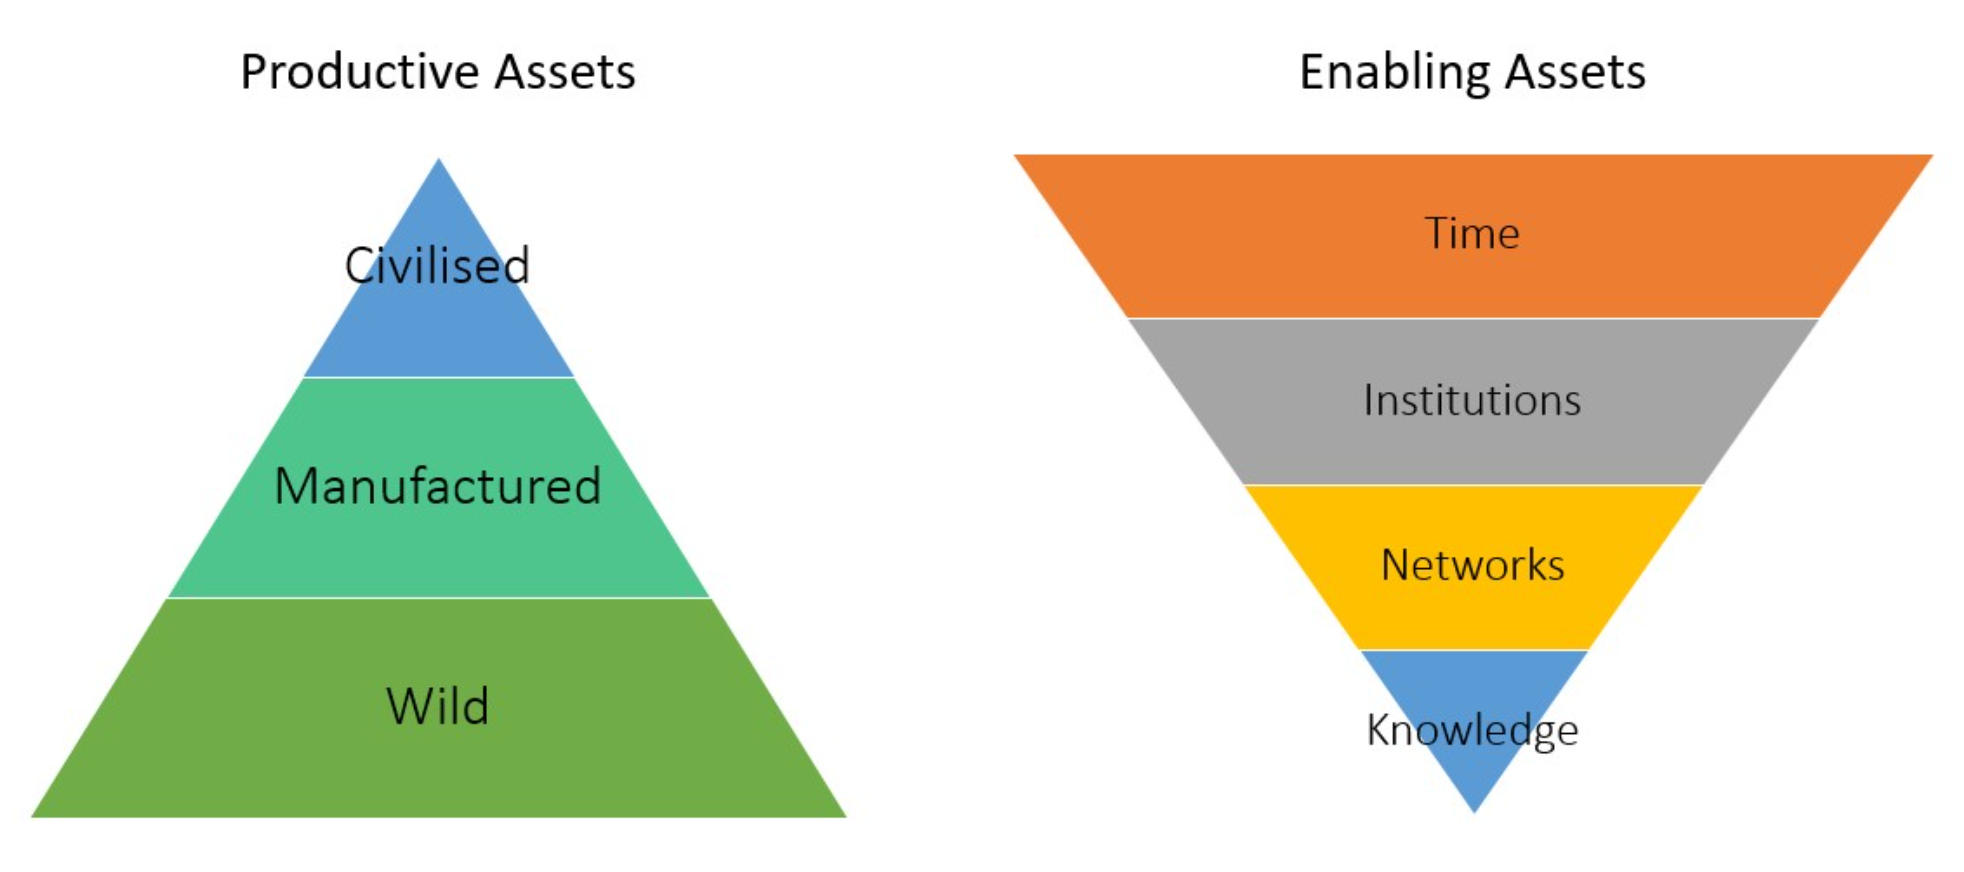
\includegraphics[width=0.75\textwidth]{productiveAssetTaxonomy.png}
\caption{Original taxonomy of influences on human well-being}
\label{Influences on well-being figure}
\end{center}
\end{figure}

Enabling assets allow society to be more precise about their influences on the physical environment, may be defined as software and possibly released for mass production. Dasgupta~\cite{pd2} also describes how enabling and production assets can exhibit different types of value:

\begin{description}
\item[Use-value:] the contribution of an asset to well-being once consumed;
\item[Intrinsic-value:] the contribution of an asset to well-being in the understanding that it exists (e.g. believing that polar bears roam free in the arctic);
\item[Option-value:] the contribution of an asset to well-being in the understanding that it may be consumed at some point in the future.
\end{description}

The attitudes and preferences that characterise a state of well-being are not defined and need to be found. Recognised methods to evaluate social attitudes and preferences are:

\begin{description}
\item[Stock markets:] Determines the values of a supply of commodities through a process of market clearing.
\item[Hedonic regression:] Determines the value of amenities by comparing house prices and the amenities available on different parcels of land to each other using regression analysis.
\item[Satisfaction/approval surveys:] Determines the level of approval from a representative sample of respondents for a particular amenity. Arrow et al.~\cite{kja1} recognised that respondent heuristics prevent valuation of an amenity using survey methods.
\end{description}

\subsubsection{Limitations}

\emph{Wild Capital}, by its very nature, does not submit to any social contract governing the state (a pre-requisite for currency).
Therefore, no human can confidently place a valuation on Wild Capital and it's contributions to well-being may be priceless.\
Cost-benefit analysis involves a number of personal assumptions that may not be particularly relevant to many people. This tool for decision-making is best suited to personal savings behaviour.
Cost-benefit analysis may be entirely inappropriate for decisions relating to \emph{essential Goods}.
Attention to distribution outliers and qualitative information is essential in assuring a just approach to personal savings goals.

\subsubsection{A Note on Perfectionism}

There is a body of thought that define the duty and obligations of individuals so as to maximise the achievement of human excellence in art, science and culture. Neitzsche~\cite{gam1} asserts:
\begin{quote}
"Mankind must work continually to produce individual great human beings---this and nothing else is the task... for the question is this: how can your life, the individual life, retain the highest value, the deepest significance?... Only by your living for the good of the rarest and most valuable specimens."
\end{quote}
However, in order to arrive at perfectionism, Rawls~\cite{jr1} asserts that we would have to attribute all parties to a prior acceptance of a certain style and aesthetic grace, and to advance the the pursuit of knowledge and the cultivation of the arts.
Whilst I believe values of excellence may be recognised, human principles need to be pursued within the limits of the principle of free association.
The coercive apparatus of states would not be used to win greater liberty or larger shares of wealth on the grounds that ones activities are of more intrinsic value.
The social resources necessary to support associations dedicated to advancing the arts, sciences and culture generally are to be won as a fair return for services rendered, or from such voluntary contributions as citizens wish to make.
Governments might limit support to cases of overcoming isolation and assurance.

\subsubsection{Demonstration, Assurance and Automation}
It is believed that the arrangements explained pose fair arguments for an equal liberty of conscience in managing the global commons.
Therefore, parties have Good grounds for adoption.
These arguments allow the choice of a regime of moral liberty and freedom of thought and belief, and of religious practice, although these may be regulated as always by state interest in public order and security.
Particular associations may be freely organised as their members wish, and could have their own internal life and discipline.
Acceptance of these limitations does not imply that public interests are in any sense superior to moral and religious interests, nor does it require that government hold indifference to religious matters or hold the right to suppress philosophical beliefs when in conflict with state affairs.
Associations represent demonstrations of different interest and may be genuine causes of further alarm in need of address.
By exercising powers in this way governments may act as the citizens' agent and satisfy their demands of a public conception of justice.
Maintenance of public order is understood as a necessary condition for everyone's achieving ends whatever they are and to fulfil their interpretation of moral and religious obligations.
A reliance on particular metaphysical doctrine or theory of knowledge is not required.
The appeal is made to common sense, plain facts and reasoning available to all.
When the denial of liberty is justified by an appeal to public order as evidenced by common sense, it is always possible to urge that the limits have been drawn incorrectly, and that experience does not justify the restriction.\

Capital budgeting involves a keen understanding of demand, so that plans can be made that develop affordable and secure supply-chains with an appropriate degree of quality assurance.
One needs to strike a balance between quality and the activities promoted through what is demanded by considering the Commonwealth Cost of Carbon.
Professional best practice would be to add the Commonwealth Cost of Carbon to expected fuel costs to budget for each items assurance requirements.
\emph{Uncaught promises} become a high priority focus area in all disciplines of engineering to improve integrated systems stability.
Any policies that stipulate objectively under-assured supply-chains runs risks of severe problems and challenge.
The consequences of failing to perform to shared understanding are simply increased levels of enforcement by states, whether judicial, or ultimately through military intervention.\

\pagebreak

\section{Continuous Integration}
To support a diverse market of complimentors platform ecosystems define boundaries for developers to integrate and offer new Features to consumers.
The Guidance and Standards that constitute these boundaries provide criteria for failure to any developer and sets a feedback-loop for learning.
Whilst \emph{Guidance} criteria are suggested as Good practice for learning practitioners, \emph{Standards} represent mandatory criteria where it appears no other reasonable option is available.
This process of development and learning to meet integration criteria is known as a process of continuous integration.
In the interest of the least-advantaged developer, continuous integration processes need offer rapid results with instructive and relevant feedback.
Developers need the ability to frequently test Features for compliance with integration requirements and indication of whether they have achieved desired outcomes.\

Guidance, Standards and review processes relating to the compliance criteria of Features may be stipulated at various stages of Feature development.
Features that exhibit a development stage need test against the relevant criteria.
These development stages are then mapped to system typologies with significantly difference requirements to establish a matrix for designating test criteria.
Test development is an important consideration of any \emph{Framework}, which sets system definitions and dependencies.
It is important that developers recognise the system typologies which are relevant to any Features.
An outline matrix for designating test criteria is shown in Table 2.

\pagebreak

\begin{table}[h]
\caption{Outline matrix designating test criteria}
	\begin{center}
		\begin{adjustbox}{angle=90}
			\begin{tabular}{| l | c | c | c | c | c | c | c |}
			\hline
			System/Stage&life&alarm&property&sensitive&personal&client&public\\
			\hline
			use&&&&&&&\\
			architecture&&&&&&&\\
			framework&&&&&&&\\
			device&&&&&&&\\
			system&&&&&&&\\
			integration&&&&&&&\\
			acceptance&&&&&&&\\
			penetration&&&&&&&\\
			market&&&&&&&\\
			\hline
			\end{tabular}
		\end{adjustbox}
	\end{center}
\label{Test matrix}
\end{table}

\pagebreak

What follows is a brief summary of some key criteria that has been established for each system typology.
The intention is that these criteria represent a pragmatic minimum for ecosystem development.
There is a reluctance to be over-prescriptive in order to maintain as extensive a system of liberty as possible.

\subsection{Life}
A life system maintains conditions of minimum decency.
The risk of life systems failure may have direct impacts upon health.
It may be perceived Professionally negligent to develop conditions that knowingly increase risk of failure in a life system without making best efforts of mitigation.\

This investigation has identified that the platform ecosystem should comply with a Hobbesian Framework for life~\cite{th1}.
Such a Hobbesian perspective leads towards a Commonwealth Cost of Carbon as an appropriate quality of life standard for this platform ecosystem at the market stage.
A Sovereign of State has ultimate responsibility to review the market of life and apply enforcement however one wills.
It is understood that no Sovereign of state has the power to enforce its rules over all life on Earth and no platform can exist without promises assured by at least one state.\

Life systems tend to be most promising when relying on simple, clear common-sense processes with little in the way of conflicting interests.
A defining feature of life systems is that integration with this alarm management platform is restricted to hard-wired digital inputs only.
This is to assure no interference from less critical systems over more permissive networks.\

The use of internet protocols is not recommended for the control of life systems.\

\subsection{Public}
System level protocols for many systems may be quite permissive to support an extensive range of options for development.
Therefore, other private systems may allow for a diverse and risky mix of traffic that may include unencrypted broadcasts.
In the interest of privacy, scalability and security public networks need only expose IPv6 protocols to the internet.
IPv6 is a preferrable standard for exposure to the public and IPSec security may be employed to encrypt traffic between permanently allocated network addresses~\cite{ipv6}.
Public networks may be fitted with internet gateways that firewall anything but specific IPv6 addresses.
Edge devices deployed on private networks may connect securely to publicly exposed devices using the transport layer security protocol over a Network Address Translation (NAT) gateway.
Network controllers can routinely test compliance of devices situated on public networks and manage network enrolment using a Framework such as FaucetSDN Device Automated Qualification~\cite{daq1}.\

A typical network configuration for a private alarm management system is illustrated in Figure~\ref{Typical Network Configuration figure}.

\begin{figure}[ht]
\begin{center}
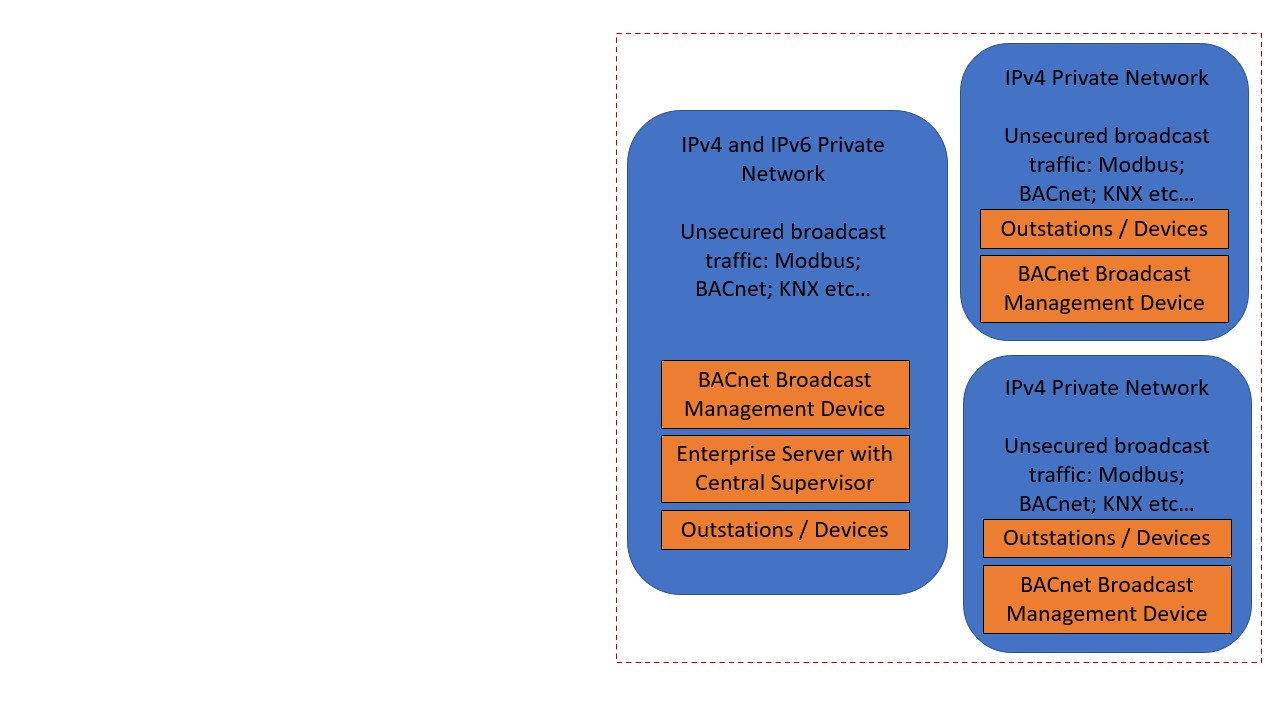
\includegraphics[width=0.75\textwidth]{typicalPrivateNetwork.jpg}
\caption{Typical network configuration for a private alarm management system}
\label{Typical Network Configuration figure}
\end{center}
\end{figure}

Following Guidance for this public network criteria.
An acceptable proposition for integration of this private network with the internet is illustrated in Figure~\ref{Integrated Network Configuration figure}.

\begin{figure}[ht]
\begin{center}
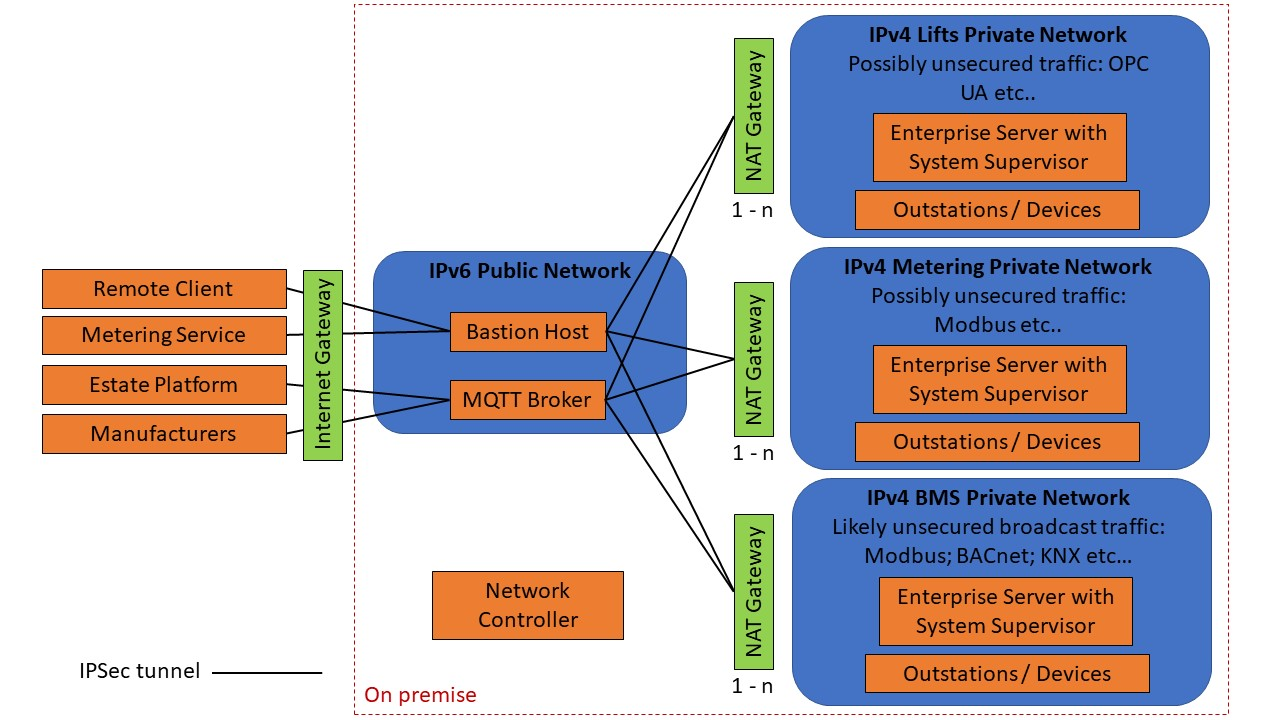
\includegraphics[width=0.75\textwidth]{acceptablePublicNetwork.jpg}
\caption{Acceptable proposition for integration of alarm management system with internet}
\label{Integrated Network Configuration figure}
\end{center}
\end{figure}

\subsection{Property}
A \emph{Property} constitutes an assured promise.
Assurance of Property is enforced by states and is subject to a states particular legal Framework.
Unless some sort of agreement has been made between states, there is no guarantee that assured promises may be understood similarly across legal Frameworks.
It is understood that the promise of intellectual Property applied to this document is assured by a Framework defined in English Law.
The present standard for the diligent management of Property are version control systems, for which Git is a popular case~\cite{git}.
With any promise of Property at any development stage, it is essential for assurance purposes to define contractual terms for its proper use under a License.
Some Property may be valuable, therefore best practice would be to encrypt any private files relating to Property with either RSA or AES data encryption Standards at rest~\cite{rsa}~\cite{aes}.

\subsection{Alarm Manager}
An alarm manager system constitutes processes that effectively discharge demands on a governance regime.
Alarm managers may take into account field observations and define procedures in order to take appropriate actions.
Alarm managers may be situated in outstations within the field and procedures defined by scripts.
This could result in alarm managers being constituted as operating computational controllers.\

Having adopted a Hobbesian perspective of the ecosystem, a Framework for alarm management defined by John Rawls, A Theory of Justice has been followed~\cite{jr1}.
Alarm management functions need to be Professionally reviewed by domain experts following this platforms Rawlsian Executive Function as a reasonable minimum.
Such alarm management reviews require understanding of market demands and demonstrations of different interests through the development of associations.
Rulings that appropriately define alarm manager operations, in the interest of timely and consistent responses, would become a promise of Property.
Promising rulings would require a system of Professional peer-reviews, with any proposed solution represented by a formal domain Ontology and compliance with the principles of this Executive Function as a minimum.
Continuous integration products, such as Jenkins or Travis CI, may be used for automated testing of software and rapid development feedback in preparation for operational releases~\cite{jenkins}~\cite{travis}.\

Alarm managers in the field may use a diverse range of network and hard-wired interfaces.
Alarms need be prioritised in a common-sense manner to direct attention:

\begin{itemize}
	\item P1, immediate action; 
	\item P2, urgent action;
	\item P3, pressing action;
	\item P4, optimisation action.
\end{itemize}

\subsection{Sensitive}
Sensitive information may be subject to assured promises that require individuals or associations to retain information in private.
Such information would likely be subject to a Framework defined by a state.
Sensitive information should be encrypted with either RSA or AES data encryption Standards at rest~\cite{rsa}~\cite{aes}.

\subsection{Personal}
Any information that may be used by organisations to identify individuals has particular relevance to personal privacy and security.
The collection, storage and use of personal information that may be used to identify individuals is enforced by states and is subject to a particular legal Framework.
Unless some sort of agreement has been made between states, there is no guarantee of common requirements across legal Frameworks.
Any personal information contained within this document is subject to a Framework defined in English Law.
Personal information that is to be assured for private use only should be encrypted with either RSA or AES data encryption Standards at rest~\cite{rsa}~\cite{aes}.

\subsection{Client}
Client applications involve the release of consumer interfaces to remote devices.
Development of releases require the adoption of a desirable Framework, such as Node.js, Flutter or Flask~\cite{node}~\cite{flutter}~\cite{flask}.
The sources of software released to client devices may have a promise of Property.
Continuous integration products, such as Jenkins or Travis CI, may be used for automated testing of source code and rapid development feedback in preparation for operational releases~\cite{jenkins}~\cite{travis}.
Client devices are typically networked over internet or serial protocols.\

\section{Operation}
The potential market of the platform ecosystem outlined here could be global.
At this time, few organisations meet the criteria that define the boundaries of the platform ecosystem defined.
This means there is considerable work to be done to signal failure to potential complimentors and initiate feedback to support an integration process.
It is also understood that the originators of this document are unlikely to be aware of all relevant information in this domain, which may result in some further change.
Therefore, an operational model is necessary.\

Within a particularly complex and generally disinterested political context, there appears a need to establish a stable and public auditable signal of thought that may be shared to establish mutual understanding.
Such a signal may become a reliable target for further development.
The following arrangements have been made to support operation of this platform ecosystem.\

\subsection{Association}
This document constitutes a public commitment of the authors to the boundaries of a platform ecosystem which is the Property of REALFEED Ltd.
REALFEED is a dormant company limited by shares registered with Companies House, a government agency of the United Kingdom.
The purpose of REALFEED is to act as an agent for one person.

\subsection{Licensing}
REALFEED has no interest in monopoly power over its markets and is keen to learn as much as possible from other agents and organisations.
The agency is keen to stay agile whilst commanding a stable knowledge base, so that it can adapt whenever necessary.
REALFEED tends to favour permissive licenses for its Property, such as the MIT license applied to this document.
It is understood that these arrangements should support conditions of fair liberty and equality of opportunity. 

\subsection{Contracts}
REALFEED is not open for appointment on a commercial basis directly.
It is an agency that intends to share knowledge in concert with other Professionals to develop mutual assured approaches for their clients.
Any popular attention paid to REALFEED would be purely a result of the companies reputation and its Good faith.

\section{Conclusion}
It has been recognised the the prevailing discussion on the governance of platform ecosystems may have contributed to global ecosystem instability in alarming ways.
The prioritisation of network effects to deliver a popular market share of consumers tends to be a common Feature.
Therefore, this document has sought to diagnose causes of instability and define new platform ecosystem boundaries for more stable outcomes.
It is understood that this has been achieved through an investigation of ethics, continuous integration processes and operations.
This investigation appreciates the differences between the \emph{states} of Locke and \emph{State} of Hobbes.
The Sovereignty of states and their role in forming civil society are recognised and this platform submits to the necessary assurance regime of a state.
However, a significant difference of this platform ecosystem to others is the acknowledgement that a society need submit to a global Sovereign of State which accounts for the condition of the Earth's ecosystem.
What follows is the use of a Hobbesian Commonwealth Cost of Carbon as an overall quality of life indicator and a Rawlsian process of alarm management.
The resulting \emph{Commonwealth of Peoples} could adopt traditional principles of justice amongst free and democratic peoples without conflict.\
Complimentors are encouraged to develop their own Features for integration with this ethical Framework.
A minimal set of criteria has been identified for complimentors to develop new Features for end-consumers.
Although these criteria are not nearly complete at this point of time, it is hoped that they prove a stable enough starting point for generating interest.\
In operation, this platform ecosystem acts as an agent for one person.
It's intentions are to share knowledge in concert with other Professionals to develop mutually assured approaches in Good faith.
Licensing of Property is highly permissive to support conditions of fair liberty and equality of opportunity.\
A public commitment by the authors to this document has now been justified, made public and is fully auditable.
Our knowledge exchange and learning process through failure continues.\

\pagebreak

\begin{thebibliography}{99}

\bibitem{bop1} Cusumano~M.A. Gawer~A. Yoffie~D.B. (2019)
\emph{The Business of Platforms}
New York, NY: HarperCollins Publishers

\bibitem{jl1} Locke~J. (1967)
\emph{Two Treatises of Government}
Cambridge: Cambridge University Press

\bibitem{rn1} Nozick~R. (1974)
\emph{Anarchy, State and Utopia}
New York, NY: Basic Books

\bibitem{th1} Hobbes~T. (1668)
\emph{Leviathan},
Oxford: Oxford University Press

\bibitem{jr2} Rawls~J. (1999)
\emph{The Law of Peoples},
Harvard: Havard University Press

\bibitem{ng1} National Geographic. (2020)
\emph{The Carbon Cycle},
Accessed 26/12/2020, available online: 
\url{https://www.nationalgeographic.org/encyclopedia/carbon-cycle/}
	
\bibitem{ba1} British Antarctic Survey (2010)
\emph{Ice Cores and Climate Change, Science Briefing},
Swindon: British Antarctic Survey
	
\bibitem{td1} Tyndall~J. (1861)
\emph{On the Absorption and Radiation of Heat by Gases and Vapours, and on the Physical Connexion of Radiation, Absorption, and Conduction. - The Bakerian Lecture},
Proceedings of the Royal Society of London; Philosophical Transactions of the Royal Society, 151, 1-36
	
\bibitem{dldh1} Harvey~D.L.D. (1993)
\emph{A Guide to Global Warming Potentials},
Energy Policy, 21(1), pp. 24-34
	
\bibitem{hj1} Hansen~J. et al. (2006)
\emph{Global Temperature Change},
Proceedings of the National Academy, 103, pp. 14,288-14,293
	
\bibitem{candm1} Cole~S., McCarthy~L. (2012)
\emph{NASA Finds 2011 Ninth-Warmest Year on Record},
Accessed 30/11/2012, available online: 
\url{http://www.nasa.gov/topics/earth/features/2011-temps.html}
	
\bibitem{ns1} Stern~N.H. (2006)
\emph{The Stern Review of the Economics of Climate Change},
Cambridge: Cambridge University Press
	
\bibitem{jr1} Rawls~J. (1971)
\emph{A Theory of Justice}
Cambridge, MA and London: Harvard University Press
	
\bibitem{rc1} Coase~R.H. (1960)
\emph{The Problem of Social Cost.},
The Journal of Law and Economics, 3, pp. 1-44
	
\bibitem{hs1} Sidgwick~H. (1877)
\emph{The Methods of Ethics}
Cambridge: Cambridge University Press
	
\bibitem{ka1} Arrow~K.J. (1963)
\emph{Social Choice and Individual Values},
New York, NY: John Wiley
	
\bibitem{km1} May~K. (1952)
\emph{A Set of Necessary and Sufficient Conditions for Simple Majority Decisions},
Econometrica, 20(4), pp. 680-684
	
\bibitem{as2} Sen~A. (1970)
\emph{Collective Choice and Social Welfare}
San Francisco: Hoden Day
	
\bibitem{jw2} Waldron~J. (1984)
\emph{Theories of Rights}
Oxford: Oxford University Press
	
\bibitem{rd1} Dworkinn~R. (1978)
\emph{Taking Rights Seriously}
London: Duckworth
	
\bibitem{np1} The Nobel Prize (2021)
\emph{William D. Nordhaus, Facts},
Accessed 04/02/2021, available online: 
\url{https://www.nobelprize.org/prizes/economic-sciences/2018/nordhaus/facts/}
	
\bibitem{g1} Press Association (2007)
\emph{Peerage for climate change economist},
Accessed 04/02/2021, available online: 
\url{https://www.theguardian.com/environment/2007/oct/19/climatechange}
	
\bibitem{bi1} Jacobs-S. Rogers~T.N. (2019)
\emph{Just 26 of the world's richest men have more combined wealth than the poorest 3.8 billion people},
Accessed 15/03/2021, available online: 
\url{https://www.businessinsider.com/worlds-richest-billionaires-net-worth-2017-6?r=US&IR=T}
	
\bibitem{fr1} Ramsey~F.P. (1928)
\emph{A Mathematical Theory of Saving.}
Economic Journal, 38(152) pp. 543-559
	
\bibitem{wc1} Cline~W.R. (1992)
\emph{The Economics of Global Warming},
Washington D.C.: Institute for International Economics
	
\bibitem{wn1} Nordhaus~W.D. (1994)
\emph{Managing the Global Commons: The Economics of Climate Change},
Cambridge, MA: MIT Press
	
\bibitem{ch1} Hope~C., Anderson~J., Wenman~P. (1993)
\emph{Policy Analysis of the Greenhouse Effect. An Application of the PAGE Model},
Energy Policy, 21, pp. 327-338
	
\bibitem{rsjt1} Tol~R.S.J. (1997)
\emph{On the Optimal Control of Carbon Dioxide Emissions: An Application of FUND},
Environmental Modelling and Assessment, 2, pp151-163
	
\bibitem{iwg1} Interagency Working Group on Social Cost of Carbon, United States Government (2013)
\emph{Technical Support Document: - Technical Update of the Social Cost of Carbon regulatory Impact Analysis - Under Executive Order 12866},
Washington D.C.: United States Government
	
\bibitem{as1} Sen~A. (1961)
\emph{On Optimizing the Rate of Saving}
Economic Journal, 71
	
\bibitem{ms1} Marglin~S.A. (1961)
\emph{The Social Rate of Discount and The Optimal Rate of Investment}
The Quaterly Review of Economics, 77(1), pp. 95-111
	
\bibitem{fh1} Hayek~F. (1944)
\emph{The Road to Serfdom}
Chicago: University of Chicago Press
	
\bibitem{eu1} European Commission (2020)
\emph{World military expenditure and weapons trade},
Accessed 26/12/2020, available online: 
\url{https://knowledge4policy.ec.europa.eu/foresight/topic/changing-security-paradigm/world-military-expenditure}
	
\bibitem{co1} co2.earth (2020)
\emph{co2.earth Are we stabilizing yet?},
Accessed 26/12/2020, available online: 
\url{https://www.co2.earth/global-co2-emissions}
	
\bibitem{oecd1} Organisation for Economic Co-operation and Development (2021)
\emph{stats.oecd.org},
Accessed 30/07/2021, available online: 
\url{https://stats.oecd.org/Index.aspx?DataSetCode=SNA_TABLE11}
	
\bibitem{nk1} Kalder~N. (1955)
\emph{An Expenditure Tax},
London: George Allen and Unwin
	
\bibitem{hp1} Prichard~H.A. (1955)
\emph{Moral Obligation},
Oxford: The Clarendon Press

\bibitem{kja1} Arrow~K.J. Solow~R.M. Portney~P. Leamer~E. Radner~R.; Schuman~H. (1993)
\emph{Report of NOAA Panel on Contingent Valuation.},
Federal Register, pp. 4601-46014
	
\bibitem{pd2} Dasgupta~P. (2001)
\emph{Valuing Goods.},
In: Human Well-Being and the Natural Environment. Oxford: Oxford University Press, pp. 122-138
	
\bibitem{pd3} Dasgupta~P. (2015)
\emph{Disregarded Capitals: What National Accounting Ignores.},
Accounting and Business Research, 45(4), pp. 122-138
	
\bibitem{gam1} Morgan~G.A. (1941)
\emph{What Nietzsche Means.}
Cambridge, MA: Harvard University Press

\bibitem{ipv6} Deering~S. Nokia~H.R. (1998)
\emph{Internet protocol, Version 6 (IPv6) Specification}
The Internet Society
\url{https://datatracker.ietf.org/doc/html/rfc2460}

\bibitem{daq1} FaucetSDN Device Automated Qualifaction Community (2022)
\emph{faucetSDN/daq}
faucetsdn
\url{https://github.com/faucetsdn/daq}

\bibitem{git} git-scm Community (2022)
\emph{faucetSDN/daq}
git
\url{https://git-scm.com/}

\bibitem{rsa} IEEE Standards Association (2000)
\emph{IEEE 1363-2000 IEEE Standard Specifications for Public-Key Cryptography}
IEEE Standards Association
\url{https://github.com/faucetsdn/daq}

\bibitem{aes} International Standards Organisation (2020)
\emph{ISO/IEC 18033-3:2010 Infomration technology - Security techniques - Encryption algorithms - Part 3: Block ciphers}
Geneva: International Standards Organisation
\url{https://www.iso.org/standard/54531.html}

\bibitem{jenkins} Jenkins Infrastructure Community (2022)
\emph{ci.jenkins.io}
ci.jenkins.io
\url{https://www.jenkins.io/}

\bibitem{travis} International Standards Organisation (2020)
\emph{Travis CI}
Leverkusen: Travis CI, GmbH
\url{https://www.travis-ci.com/}


\bibitem{node} OpenJS Foundation (2022)
\emph{node.js}
OpenJS Foundation
\url{https://nodejs.org/en/}

\bibitem{flutter} Flutter (2022)
\emph{Flutter}
Mountain View, CA: Google 
\url{https://flutter.dev/}

\bibitem{flask} Pallets Community (2022)
\emph{Flask web development, one drop at a time}
palletsprojects
\url{https://flask.palletsprojects.com}

\end{thebibliography}

\pagebreak

\section{Annex: Public Access to Digital Assurance Ontology}

\url{https://github.com/realfeed/manifesto/blob/main/digitalAssurance.xml}

\end{document}  
